\usepackage{listings}\section{ПРОГРАММА И МЕТОДИКА ИСПЫТАНИЙ}
\label{sec:testing}

%В разделе, посвященном программе и методике испытаний, описываются внутренние (если самотестирование заложено в программу)
%и внешние средства тестирования. Могут использоваться как оригинальные, так и стандартные тесты.
%Рассматриваются способы проверки  надежности (устойчивости, стабильности и т. д.) разработанной программы в различных режимах,
%включая много-пользовательский и многозадачный режимы, а также  корректность обработки входных, промежуточных и выходных данных, в том числе:
%в области граничных значений допустимых диапазонов, заведомого неправильных данных, фай-лов  большого  размера.
%Для  каждого  из  тестов  приводятся  исходные  данные, параметры и результаты

В данном разделе рассмотрено тестирование разработанной системы.
Его необходимо проводить перед выпуском продукта или системы с целью выявления ошибок и их устранения, для проверки соответствия продукта
заявленным требованиям, оценки качества работы разработчиков, получения информации о сложности системы и ее характеристиках.
Тестирование обеспечивает безопасность кода при командной работе, помогает в создании наилучшей
архитектуры, улучшает качество кода, упрощает исправление ошибок и экономит денежные средства организации.

\subsection{Методологии тестирования}
Методологии тестирования представляют собой набор принципов, подходов и практик,
которые помогают разработчикам и тестировщикам обеспечить высокое качество программного обеспечения.
Они определяют стратегии и процессы, используемые для тестирования приложений,
и включают в себя различные методы и техники, направленные на выявление ошибок и дефектов.

Одной из важных методологий тестирования является «пирамида тестирования», которая приведена на рисунке~\ref{fig:testing:testing_piramide}.
Данный подход описывает структуру тестов в виде пирамиды, где на нижних уровнях располагаются более
простые и быстрые в исполнении тесты, а на верхних — более сложные и медленные.
Такая структура позволяет достичь баланса между охватом различных типов тестирования и затратами на его проведение.

\begin{figure}[ht]
    \centering
    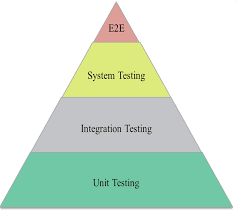
\includegraphics[width=.6\linewidth]{images/testing_piramide}
    \caption{Пирамида тестирования}
    \label{fig:testing:testing_piramide}
\end{figure}

%На нижнем уровне пирамиды находятся модульные тесты.
%Они проверяют отдельные компоненты приложения, такие как функции или классы,
%и обеспечивают быструю обратную связь о работоспособности кода.
%Следующий уровень — интеграционные тесты, которые проверяют взаимодействие между различными компонентами приложения.
%На верхнем уровне располагаются системные тесты, которые проверяют работу приложения в целом и его соответствие требованиям заказчика или спецификации.
%Пирамида тестирования призвана обеспечить баланс между широким охватом функциональности приложения и эффективным использованием
%ресурсов на проведение тестирования.
%Этот подход позволяет сосредоточить основное внимание на низкоуровневых, более надежных и быстрых тестах,
%в то время как более высокоуровневые, медленные и дорогостоящие тесты используются в меньшем объеме, но обеспечивают проверку работы
%приложения в реальных условиях использования.

\subsection{Технологии для тестирования}\label{subsec:testing:testing-technologies}

Веб-приложение трейдинговая платформа тщательно тестировалось в процессе разработки.
Для проведения тестирования язык программирования Python имеет встроенную библиотеку unittest.
Для тестирования веб-приложения трейдинговая платформа была выбрана библиотека pytest.
Данная библиотека является оберткой над стандартной библиотекой unittest, однако предоставляет куда больший функционал для тестирования.

Pytest обладает более простым и интуитивно понятным синтаксисом по сравнению с unittest.
Он требует меньше кода для написания тестов, что ускоряет процесс написания тестов.
Pytest предоставляет множество встроенных функций и возможностей для тестирования, таких как
автоматическое обнаружение тестов, параметризованные тесты, фикстуры.

Это позволяет сделать написание и запуск тестов более гибким и эффективным.

Pytest также предоставляет более информативные отчеты об ошибках по сравнению с unittest.
Они содержат более подробную информацию о том, что именно пошло не так в тесте, что облегчает отладку и исправление ошибок.

Pytest предоставляет возможность расширять его функциональность с помощью плагинов.
Это позволяет добавлять дополнительные возможности, такие как поддержка новых типов тестов, интеграция с другими инструментами.
Одним из таких плагинов является библиотека pytest-django, которая специализируется на написании тестом для приложений, написанных с использованием фреймворка Django.
Одним из преимуществ использования данной библиотеки является фикстура~\lstinline{django_db}, которая создаёт базу данных для использования в тестах.

Основными элементами при написании тестов с использованием библиотеки pytest являются:
\begin{enumerate_num}
    \item Фикстура.
    \item Мок.
    \item Патч.
\end{enumerate_num}

Проверка работоспособности системы была проведена с помощью большого количества тестов, поэтому на рассмотрение вынесено тестирование самых важных алгоритмов и функций.

\subsection{Вспомогательные фикстуры}\label{subsec:testing:fixtures}
Фикстуры, упомянутые в разделе~\ref{subsec:testing:testing-technologies}~являются функциями, однако не требуют вызова при написании тестов.
В зависимости от области, которая указывается при описании фикстур, они вызываются автоматически.
Если область не указана, то фикстуры будут выполняться при их передаче в качестве параметров внутри функций-тестов.

Для указания интерпретатору информации о том, что функция является фикстурой, используется декоратор \lstinline{@pytest.fixture}.

Область видимости фикстур связана с расположением файла conftest.py, в котором они описываются.
Импортировать фикстуры для их указания в качестве аргументов функции не требуется.

\subsubsection{Вспомогательные фикстуры Django микросервиса}

Фикстуры, указанные ниже, описаны в файле conftest.py, который находится в корневой директории Django проекта,
что позволяет использовать их в тестах любого из модулей.

Для написания тестов требуются данные, которые будут храниться в виде записей в тестировочной базе данных.
Для инициализации записи в каждой таблице были описаны следующие фикстуры, которые были помечены при помощи декоратора~\lstinline{@pytest.mark.django_db}:
\begin{enumerate_num}
    \item trader.
    Данная фикстура создаёт и возвращает объект класса~\lstinline{User}, с правами доступа~\lstinline{trader}.
    Она также сохраняет запись в тестировочной базе данных, иннициализируя поля
    ~\lstinline{username},~\lstinline{first_name},~\lstinline{last_name},~\lstinline{email},~\lstinline{cash},~\lstinline{role} и~\lstinline{is_email_verified}.
    \item analyst.
    Данная фикстура создаёт и возвращает объект класса~\lstinline{User}, с правами доступа~\lstinline{analyst}.
    Она также сохраняет запись в тестировочной базе данных, иннициализируя поля
    ~\lstinline{username},~\lstinline{first_name},~\lstinline{last_name},~\lstinline{email} и~\lstinline{role}.
    \item admin.
    Данная фикстура создаёт и возвращает объект класса~\lstinline{User}, с правами доступа~\lstinline{admin}.
    Она также сохраняет запись в тестировочной базе данных, иннициализируя поля
    ~\lstinline{username},~\lstinline{first_name},~\lstinline{last_name},~\lstinline{email} и~\lstinline{role}.
    \item currency.
    Данная фикстура создаёт и возвращает объект класса~\lstinline{Currency}.
    Она также сохраняет запись в тестировочной базе данных, иннициализируя поля
    ~\lstinline{name},~\lstinline{info},~\lstinline{rate} и~\lstinline{role}.
    \item transaction.
    Данная фикстура создаёт и возвращает объект класса~\lstinline{Transaction}, которая привязана к пользователю и валюте,
    инициализированных при помощи фикстур~\lstinline{trader} и ~\lstinline{currency}.
    Она также сохраняет запись в тестировочной базе данных, иннициализируя поля
    ~\lstinline{rate},~\lstinline{count},~\lstinline{user} и~\lstinline{currency}.
\end{enumerate_num}

Также, так как авторизация и аутентификация основана на промежуточном ПО, требуется описать фикстуры,
которые будут возвращать JWT, привязанный к пользователю с каждым правом доступа, для их непосредственной передачи при тестировании API.
Такими фикстурами являются~\lstinline{trader_token},~\lstinline{analyst_token} и~\lstinline{admin_token}, возвращающие токены с правами
доступа трейдера, аналитика и администратора соответственно.

%\subsubsection{Вспомогательные фикстуры FastAPI микросервиса}
%...

\subsection{Тесты модуля \moduleAuth}\label{subsec:testing:moduleauth}

Первая группа тестов посвещена модулю \moduleAuth.
Для тестирования модуля аутентификации требуется создать фикстуры, которые будут возвращать неправильные JWT.
Нижеупомянутые фикстуры описываются в файле conftest.py, который находится в директории authentication,
что позволяет использовать их в тестах соответствующего модуля.

Для возврата полностью неправильного JWT определена фикстура~\lstinline{invalid_token}.

Для возврата JWT, время жизни которого истекло, используется фикстура ~\lstinline{expired_tokens}.
Данная фикстура возвращает правильную пару токенов:
~\lstinline{access_token} и~\lstinline{refresh_token}, однако устанавливает параметр ~\lstinline{exp} в значение, которое делает токены истекшими.

\subsubsection{Тестирование промежуточного ПО}
При тестировании промежуточного ПО были описаны две фикстуры для локального использоване внутри файла с тестами.
Фикстуры~\lstinline{rf} и~\lstinline{jwt_middleware} создают и возвращают объекты классов~\lstinline{RequestFactory} и ~\lstinline{JWTAuthenticationMiddleware} соответственно.
Первая их них нужна для вызова запроса к одному из эндпоинтов, а вторая для непосредственного вызова метода~\lstinline{process_request} класса~\lstinline{JWTAuthenticationMiddleware}.

Все упомянутые тесты обернуты в декоратор ~\lstinline{@pytest.mark.django_db}, так как при декодировании JWT промежуточное ПО сверяет данные из токена с данными, хранящимися в базе данных.
Ее тестирование производилось с помощью описанных далее функций.

Тест \lstinline{test_valid_token} принимает аргументами локальные фикстуры~\lstinline{rf},~\lstinline{jwt_middleware} и фикстуру ~\lstinline{trader}.
Далее при помощи фикстуры~\lstinline{rf} формируется объект класса ~\lstinline{WSGIRequest}, который является запросом к эндпоинту, передавая в заголовке запроса~\lstinline{AUTHORIZATION} правильный JWT, сформированный на основании данных ~\lstinline{trader}.
После этого происходит вызов метода~\lstinline{process_request}, куда параметром передатся уже сформированный объект класса ~\lstinline{WSGIRequest}.
Как было упомянуто в разделе~\ref{subsubsec:func:module-authentication}, данный метод лишь модифицирует переданный ему объект класса ~\lstinline{WSGIRequest}.
Далее происходит сравнение исходного никнейма пользователя~\lstinline{trader} и того, который находится внутри объекта класса~\lstinline{WSGIRequest} -- \lstinline{request.user.username}

Аналогично работают тесты~\lstinline{test_expired_token},~\lstinline{test_invalid_token} и ~\lstinline{test_no_token}, однако они имеют другие условия для проверки.
Тест~\lstinline{test_expired_token} проверяет поведение промежуточного ПО на проверку токена, время жизни которого истекло.
Он проверяет, является ли статус код~\lstinline{response.status_code} из ответа статусом ~\lstinline{status.HTTP_401_UNAUTHORIZED}.
Данный тест также проверяет что текс сообщения ~\lstinline{response.content} ответа соответствует значению~\lstinline{"Token has expired"}.

Тест~\lstinline{test_invalid_token} проверяет поведение промежуточного ПО на проверку токена, который не соответствует заданной структуре JWT.
Он проверяет, является ли пользователь~\lstinline{request.user} из ответа пользователем с правами доступа ~\lstinline{AnonymousUser}.

Тест~\lstinline{test_invalid_token} проверяет поведение промежуточного ПО на обработку запроса, который не содержит токена в заголовке .

%Тестирование данных эндпоинтов разбито на классы, каждый из которых реализует в тесты для каждого из эндпоинтов.
%К данным классам относятся классы~\lstinline{TestJWTObtainPairEndpoint},
%~\lstinline{TestJWTRefreshPairEndpoint},~\lstinline{TestSendEmailToResetPassword},
%~\lstinline{TestSendSecretCodeToResetPassword} и~\lstinline{TestVerifyEmailMixin}.
%Данные классы реализуют тесты для эндпоинтов в соответствии с их названиями.

\subsubsection{Тестирование представления TokenObtainPairViewSet}

Тесты, описанные в классе~\lstinline{TestJWTObtainPairEndpoint} проверяют поведение эндпоинта~\lstinline{TokenObtainPairViewSet} на
разные параметры, переданные в запросе.
Тест~\lstinline{test_success_token_obtain_pair_view} проверяет поведение эндпонта при передаче правильных параметров в запрос.
Он проверяет соответствие статуса ответа~\lstinline{response.status_code} статусу ~\lstinline{response.status.HTTP_200_OK}.
Также данный тест проверяет наличие пары токенов~\lstinline{access_token} и~\lstinline{refresh_token} в теле ответа~\lstinline{response.data}.

Тесты~\lstinline{test_invalid_password_token_obtain_pair_view} и
~\lstinline{test_invalid_username_token_obtain_pair_view} проверяют поведение эндпоинта на
неправильно переданные в запрос параметры~\lstinline{password} и~\lstinline{username} соответственно.
Данные тесты проверяют соответствие статуса ответа~\lstinline{response.status_code} статусу ~\lstinline{response.status.HTTP_400_BAD_REQUEST}.
Также они проверяют отсутствие пары токенов~\lstinline{access_token} и~\lstinline{refresh_token} в теле ответа~\lstinline{response.data}.
% МЕТОД ПОСТ ОНЛИИИИИИИИИИИИИИИИИИИИИИИИИИИИИИИИИИИИИИИИИ!!!!!!!!!!!!!!!!!!!!!!!!!!!!!!!!!!

\subsubsection{Тестирование представления TokenRefreshViewSet}

Тесты, описанные в классе~\lstinline{TestJWTRefreshPairEndpoint} проверяют поведение эндпоинта~\lstinline{TokenRefreshViewSet} на
разные параметры, переданные в запросе, аналогично тестам, описанным в классе~\lstinline{TestJWTObtainPairEndpoint}.

\subsubsection{Тестирование представления SendEmailToResetPassword}
~\lstinline{send_smtp_email_mock}


\subsubsection{Тестирование представления SendSecretCodeToResetPassword}
~\lstinline{}


\subsubsection{Тестирование представления VerifyEmailMixin}
~\lstinline{}


%
%\subsubsection{Тестирование}
%
%Первая группа тестов посвящена модулю \moduleCfg. Важным алгоритмом системы является
%функция разбора \cid-файла \lstinline{conf_parseGooseIntAddr_private}.
%
%Тест \lstinline{test_parseGooseIntAddr_confusedParam} принимает некорректные строки \cid-файла с перепутанной последовательностью правильно заполненных элементов \lstinline{source}, \lstinline{mac}, \lstinline{goId}, \lstinline{appId}, \lstinline{confRev}, \lstinline{vars}.
%В тесте создается корректный вариант строки и вызывается проверяемая функция разбора строки \cid-файла.
%Все входные неправильные строки теста сравниваются с ней, в случае совпадения тест проходит, при несоответствии~-- возвращает номер строки и вспомогательное сообщение  об ошибке.
%
%Тест \lstinline{test_parseGooseIntAddr_errorBrackets} принимает некорректные строки \cid-файла с ошибочным количеством символов <<\}>> или <<\{>>. Также скобки могут быть расставлены в неподходящем порядке, что тоже является ошибкой. В тесте происходит вызов проверяемой функции разбора строки \cid-файла. Проверяется возвращаемое значение на \lstinline{NULL}: если совпадает, то тест возвращает номер строки и вспомогательное сообщение об ошибке, в обратном случае он проходит.
%
%Тест \lstinline{test_parseGooseIntAddr_good} принимает правильную строку \cid-файла. Создается корректный вариант строки и вызывается проверяемая функция разбора строки \cid-файла в тесте. Входная правильная строка сравнивается с созданной, в случае совпадения тест проходит, при несоответствии~-- возвращает номер строки и вспомогательное сообщение  об ошибке.
%
%Тест \lstinline{test_parseGooseIntAddr_errorSource} принимает некорректные строки \cid-файла с ошибочным параметром \lstinline{source}, все остальные значения верны. В тесте происходит вызов функции разбора строки \cid-файла. Проверяется возвращаемое значение на \lstinline{NULL}: если совпадает, то тест возвращает номер строки и вспомогательное сообщение об ошибке, в обратном случае он проходит.
%
%Тест \lstinline{test_parseGooseIntAddr_correctSource} принимает правильные строки \cid-файла с всевозможным значением параметра \lstinline{source}, все остальные значения верны тоже. В тесте создается корректный вариант строки для каждого варианта принимаемой строки и вызывается функция разбора строки \cid-файла. Все входные строки сравниваются с созданными строками в тесте. В случае совпадения он проходит, при несоответствии~-- возвращает номер строки и вспомогательное сообщение  об ошибке.
%
%Тест \lstinline{test_parseGooseIntAddr_errorMacAddress} принимает некорректные строки \cid-файла с ошибочным параметром \lstinline{mac}, все остальные значения верны. В тесте происходит вызов функции разбора строки \cid-файла. Проверяется возвращаемое значение на \lstinline{NULL}: если совпадает, то тест возвращает номер строки и вспомогательное сообщение об ошибке, в обратном случае он проходит.
%
%Тест \lstinline{test_parseGooseIntAddr_errorGoId} принимает некорректные строки \cid-файла с ошибочным параметром \lstinline{goId}, все остальные значения верны. В тесте происходит вызов функции разбора строки \cid-файла. Проверяется возвращаемое значение на \lstinline{NULL}: если совпадает, то тест возвращает номер строки и вспомогательное сообщение об ошибке, в обратном случае он проходит.
%
%Тест \lstinline{test_parseGooseIntAddr_errorConfRev} принимает некорректные строки \cid-файла с ошибочным параметром \lstinline{confRev}, все остальные значения верны. В тесте происходит вызов функции разбора строки \cid-файла. Проверяется возвращаемое значение на \lstinline{NULL}: если совпадает, то тест возвращает номер строки и вспомогательное сообщение об ошибке, в обратном случае он проходит.
%
%Тест \lstinline{test_parseGooseIntAddr_correctConfRev} принимает правильную строку \cid-файла со всевозможным значением параметра \lstinline{confRev}. Создается корректный вариант строки для каждой из входных строк и вызывается функция разбора строки \cid-файла в тесте. Входная строка сравнивается с созданной, в случае совпадения тест проходит, при несоответствии~-- возвращает номер строки и вспомогательное сообщение  об ошибке.
%
%Тест \lstinline{test_parseGooseIntAddr_confRevNull} принимает правильную строку \cid-файла c нулевым значением параметра \lstinline{confRev}. Создается корректный вариант строки и вызывается функция разбора строки \cid-файла в тесте. Входная строка сравнивается с созданной, в случае совпадения тест проходит, при несоответствии~-- возвращает номер строки и вспомогательное сообщение об ошибке.
%
%Тест \lstinline{test_parseGooseIntAddr_errorFormating} принимает некорректные строки \cid-файла с ошибочным количеством символов <<,>>, <<.>> или <<;>>. В тесте происходит вызов функции разбора строки \cid-файла. Проверяется возвращаемое значение на \lstinline{NULL}: если совпадает, то тест возвращает номер строки и вспомогательное сообщение об ошибке, в обратном случае он проходит.
%
%Тест \lstinline{test_parseGooseIntAddr_errorAppId} принимает некорректные строки \cid-файла с ошибочным параметром \lstinline{appId}, все остальные значения верны. В тесте происходит вызов функции разбора строки \cid-файла. Проверяется возвращаемое значение на \lstinline{NULL}: если совпадает, то тест возвращает номер строки и вспомогательное сообщение об ошибке, в обратном случае он проходит.
%
%Тест \lstinline{test_parseGooseIntAddr_correctAppId} принимает правильную строку \cid-файла со всевозможным значением параметра \lstinline{appId}. Создается корректный вариант строки для каждой из входных строк и вызывается функция разбора строки \cid-файла в тесте. Входная строка сравнивается с созданной, в случае совпадения тест проходит, при несоответствии~-- возвращает номер строки и вспомогательное сообщение об ошибке.
%
%Тест \lstinline{test_parseGooseIntAddr_appIdNull} принимает правильную строку \cid-файла c нулевым значением параметра \lstinline{appId}. Создается корректный вариант строки и вызывается функция разбора строки \cid-файла в тесте. Входная строка сравнивается с созданной, в случае совпадения тест проходит, при несоответствии~-- возвращает номер строки и вспомогательное сообщение об ошибке.
%
%Тест \lstinline{test_parseGooseIntAddr_errorVars} принимает некорректные строки \cid-файла с ошибочным количеством параметров \lstinline{vars} или неправильными значениями этих параметров. В тесте происходит вызов функции разбора строки \cid-файла. Проверяется возвращаемое значение на \lstinline{NULL}: если совпадает, то тест возвращает номер строки и вспомогательное сообщение об ошибке, в обратном случае он проходит.
%
%Тест \lstinline{test_parseGooseIntAddr_vars1} принимает правильную строку \cid-файла с одним параметром \lstinline{vars} с корректным значением. В тесте происходит вызов функции разбора строки \cid-файла и создание строки для сравнения. Входная строка сравнивается с созданной, в случае совпадения тест проходит, при несоответствии~-- возвращает номер строки и вспомогательное сообщение об ошибке.
%
%Тест \lstinline{test_parseGooseIntAddr_vars2} является аналогом предыдущего
%теста, как и \lstinline{test_parseGooseIntAddr_vars3}.
%Они различаются только количеством принимаемых параметров \lstinline{vars} и проверяют корректность
%обработки нескольких похожих блоков.
%
%Вспомогательной функцией модуля конфигурации является функция преобразования MAC-адреса в правильный формат~-- \lstinline{test_convertMacToCorrectFormat}. Ниже описаны тесты для ее тестирования.
%
%Тест \lstinline{test_convertMacToCorrectFormat_correct} принимает правильные MAC-адреса для преобразования в нужный формат. Они содержат корректные символы, строки полные, без лишних элементов. Тест выделяет буфер под новый преобразованный адрес и вызывает функцию конвертации. Проверяется возвращаемое значение на \lstinline{true}: если произошла ошибка преобразования, то тест возвращает номер строки и вспомогательное сообщение об ошибке, в обратном случае он проходит.
%
%Тест \lstinline{test_convertMacToCorrectFormat_error} принимает некорректные MAC-адреса для преобразования в нужный формат. Они содержат ошибочные символы, неполные строки, лишние элементы. Тест выделяет буфер под новый преобразованный адрес и вызывает функцию конвертации. Проверяется возвращаемое значение на \lstinline{true}: если произошла ошибка преобразования, то тест возвращает номер строки и вспомогательное сообщение об ошибке, в противном случае он проходит.
%
%Тест \lstinline{test_convertMacToCorrectFormat_upper} принимает корректные MAC-адреса для преобразования в нужный формат, состоящие только из прописных букв. Он выделяет буфер под новый преобразованный адрес и вызывает функцию конвертации. Проверяется возвращаемое значение на \lstinline{true}: если произошла ошибка преобразования, то тест возвращает номер строки и вспомогательное сообщение об ошибке, в противном случае он проходит. Также проверяется преобразованный адрес: в тесте создаются ожидаемые результаты преобразованных MAC-адресов и производится сравнение с результатом работы функции.
%
%Тесты \lstinline{test_convertMacToCorrectFormat_goodNumber} и \lstinline{test_convertMacToCorrectFormat_lower} работают аналогично предыдущему: принимают корректные MAC-адреса для преобразования в нужный формат, состоящие только из  цифровых значений или  строчных букв соответственно.
%
%\subsection{Тесты модуля \moduleRecvPackets}
%
%Модуль \moduleRecvPackets\ протестирован особенно тщательно в связи с возлагаемой на него логической нагрузкой и важностью занимаемого места в системе. Проверена как внутренняя работа, так и внешнее взаимодействие с другими модулями системы. Некоторые тесты невозможно было написать только для этого модуля, поэтому они охватывают сразу несколько модулей.
%
%\subsubsection{Основная бизнес-логика модуля}
%
%Тест \lstinline{test_invalidDstMacAddr} открывает вспомогательную тестовую очередь, создает буфер с отправляемым модулю пакетом для дальнейшего сравнения.
%Созданный GOOSE-пакет с некорректным  MAC-адресом назначения (такой адрес, который не совпадает с заявленной конфигурацией ожидаемого пакета) посылается в модуль. По завершении теста ожидается, что память, в которую модуль должен был разложить данные, не изменилась. Если данное условие выполняется, то тест завершается успехом, в обратном случае ожидается ошибка.
%
%Тест \lstinline{test_correctDstMacAddr} открывает вспомогательную тестовую очередь, создает буфер с отправляемым модулю пакетом для дальнейшего сравнения.
%Созданный GOOSE-пакет с корректным  MAC-адресом назначения посылается в модуль. По завершении теста ожидается, что память, в которую модуль должен был разложить данные, изменилась и соответствует заявленному пакету. Если данное условие выполняется, то тест завершается успехом, в обратном случае ожидается ошибка.
%
%Выше описаны два теста для MAC-адреса назначения. Аналогичные тесты были проведены для следующих параметров как \lstinline{goCbRef} и \lstinline{appId}.
%Тесты \lstinline{test_invalidGoCbRef}, \lstinline{test_correctGoCbRef}, \lstinline{test_invalidAppId} и \lstinline{test_correctAppId} по завершении проверяют наличие или отсутствие изменений в памяти и возвращают соответствующий результат.
%
%Тест \lstinline{test_correctPacket} принимает пакет со всеми правильно заполненными полями и с максимальной заполненностью. Основная задача данного теста~-- выяснить, справляется ли модуль с пакетами максимального размера. Проверка происходит по количеству измененных байт в памяти, а также по наличии новых данных, которые соответствуют заявленным.
%
%Тест \lstinline{test_confuseNestings} работает с корректным пакетом, но с перепутанными между собой уровнями вложенности. Проверяется, способен ли модуль правильно обрабатывать такие пакеты. Это происходит по количеству измененных байт в памяти, а также по наличии новых правильно разложенных данных, которые соответствуют заявленным.
%
%\subsubsection{Входные параметры модуля}
%
%У каждого модуля системы есть входные параметры, такие как приоритет потоков, глубина очередей, максимальный размер передаваемых и принимаемых через очередь сообщений. В следующей подгруппе тестов происходит проверка этих параметров.
%
%Тест \lstinline{test_gooseInput_allParamNULL} принимает все вышеописанные параметры нулевыми. Вызывается функция инициализации модуля, проверяется, что система не сломалась и функция вернула \lstinline{GOOSE_INPUT_RET_CODE_INIT_ERROR}.
%
%Тест \lstinline{test_gooseInput_messageSize0} принимает в качестве параметра нулевое значение размера сообщения для передачи и приема. Вызывается функция инициализации модуля, проверяется, что она вернула \lstinline{GOOSE_INPUT_RET_CODE_INIT_ERROR} и система не сломалась.
%
%Тест \lstinline{test_gooseInput_messageSize} принимает в качестве параметров корректные граничные значения размера сообщения для передачи и приема. Вызывается функция инициализации модуля, проверяется, что она вернула \lstinline{GOOSE_INPUT_RET_CODE_OK} и система работает корректно.
%
%Тесты \lstinline{test_gooseInput_depth0} и \lstinline{test_gooseInput_depth} выполняются аналогично вышеописанным тестам с размером сообщения, только проверяется глубина очереди.
%
%Есть группа тестов на приоритеты потоков, которых три в системе. Тесты основного потока \lstinline{test_prioProcTaskValid}, потока подписок \lstinline{test_prioSubscriptionTaskValid} и потока, ответственного за временные рамки работы системы, \lstinline{test_prioTimeProcessTaskValid} принимают граничные корректные значения приоритетов задач и ожидают, что вызываемая функция инициализации модуля вернет \lstinline{GOOSE_INPUT_RET_CODE_OK} и система работает корректно.
%
%Тесты основного потока \lstinline{test_prioProcTaskInvalid}, потока подписок  \lstinline{test_prioSubscriptionTaskInvalid} и потока, ответственного за временные рамки работы системы, \lstinline{test_prioTimeProcessTaskInvalid} принимают некорректные значения приоритетов задач и ожидают, что вызываемая функция инициализации модуля вернет \lstinline{GOOSE_INPUT_RET_CODE_INIT_ERROR}.
%
%\subsection{Тесты модуля \moduleProcessPackets}
%
%При обработке пакета используются множество алгоритмов перед его непосредственным помещением в память. Как было указано ранее, пакеты могут содержать информацию с данными разных типов. Основной задачей этого раздела является тестирование всевозможных вариантов данных, их обработки и преобразования.
%
%Все строки делятся на две группы: у которых длина больше 64 байт и у которых она меньше или равна этому значению. Внутри системы используются собственные типы данных, упрощающих работу модулей. На этапе тестирования достаточно знать, что длина сообщения соответствует одной из двух вышеописанных групп.
%
%Тест  \lstinline{test_checkStringLess64Size} принимает пакеты со строковой информацией до 64 байт включительно, выполняет проверку преобразования данных, корректного разложения их память. Проверяется область памяти, куда должны были записаться новые данные. В случае успеха тест пройден корректно, в противном случае ожидается ошибка.
%
%Тест  \lstinline{test_checkStringMore64Size} принимает пакеты со строковой информацией более 64 байт, выполняет проверку преобразования данных, корректного разложения их память. Проверяется область памяти, куда должны были записаться новые данные. В случае успеха тест пройден корректно, в противном случае ожидается ошибка.
%
%Тесты для типов Integer, Boolean, Unsigned,
%Dp, Quality и UtcTime выполняются аналогично вышеописанным тестам со строковыми типами данных. Также выполняется преобразования в типы системы и запись информации в память. Для текущих типов в модуле соответствуют конкретные аналоги, вариативность не поддерживается. При ошибке формата пришедших данных пакет отбрасывается. В случае успеха проверяется размер записанных в память данных, а также ее наполнение, которое должно соответствовать заявленному.
%
%\subsection{Покрытие исходного кода}
%
%Статистика помогает произвести оценку масштаба того или иного явления, а также разработать систему методов для анализа и изучения.
%
%Тестовое покрытие -- это «плотность» покрытия тестами выполняемого программного кода или требований к нему. Чем больше тестовых вариантов проверено, тем выше процент покрытия. Выделяются следующие типы тестового покрытия:
%
%\begin{itemize}
%    \item покрытие требований;
%    \item покрытие программного кода;
%    \item проверочное покрытие на основе проанализированных данных потока управления.
%\end{itemize}
%
%Все типы тестового покрытия не только направлены на улучшение качества создания и проверки программного обеспечения, но и существенным образом повышают уровень удовлетворенности продуктом со стороны заказчика.
%
%Для вычисления процента покрытия в данном проекте использовалась программа gcov, которая входит в состав набора инструментов GCC. Она сообщает, какой процент
%строк исходного кода был проверен как для конкретной функции, так и для файла, целого модуля и даже системы, какие строки кода фактически выполнялись с контрольными примерами для достижения удовлетворительного охвата и ожидаемой работы, сколько времени длились вычисления для каждого фрагмента кода, что помогает в процессе оптимизации. Такого рода информация позволяет сделать выводы о необходимости более тщательного тестирования, если процент, возвращаемый программой, не соответствует
%ожиданиям.
%
%\begin{table}[ht]
%    \caption{Статистика покрытия тестами системы}
%    \label{table:testing:codeCoverageStats}
%    \begin{tabular}{| >{\raggedright}m{0.6\textwidth}
%                    | >{\centering\arraybackslash}m{0.347\textwidth}|}
%        \hline
%        \centering Название модуля & Покрытие, $\%$ \\
%
%        \hline
%        Модуль \moduleCfg & $ 91 $ \\
%
%        \hline
%        Модуль \moduleRecvPackets & $ 76 $ \\
%
%        \hline
%        Модуль \moduleProcessPackets & $ 84 $ \\
%
%        \hline
%    \end{tabular}
%\end{table}
%
%Высокие показатели в таблице~\ref{table:testing:codeCoverageStats} свидетельствуют об ответственном подходе к тестированию, грамотной постановке задачи для разработки системы. Однако результаты не равняются $ 100 \ \%$, что объясняется невозможностью или повышенной сложностью эмуляции работы функций-заглушек других модулей, невнимательностью тестировщиков, ограниченностью во времени работы, отказом заказчика от части тестов.
